\documentclass[hyperref,oneside]{book}

\usepackage{MathBF}
\usepackage{geometry}
\geometry{a4paper,scale=0.8}
%\geometry{a5paper,scale=0.8}
\usepackage{newtxtext,newtxmath}
\usepackage{amsmath,mathrsfs,amsfonts,amssymb}
\usepackage{bm}
\usepackage{esint}
\usepackage{tikz}
\usepackage{graphics}
\usepackage[UTF8,scheme=chinese,heading=true]{ctex}

%\everymath{\displaystyle}

\newcommand{\xiti}{\section*{\large{习\qquad题}}}
\newcommand\thmref[1]{引理~\ref{#1}}
\newtheorem{yinli}{引理}
\newtheorem{example}{例}
\newenvironment{proof}{\par\noindent\textbf{证明\quad}}{\hfill$\Box$\quad\par}
\newenvironment{Definition}{\par\noindent\textbf{定义\quad}}


\renewcommand{\leq}{\leqslant}
\renewcommand{\geq}{\geqslant}

\begin{document}
    %封面设置
    \begin{titlepage}
        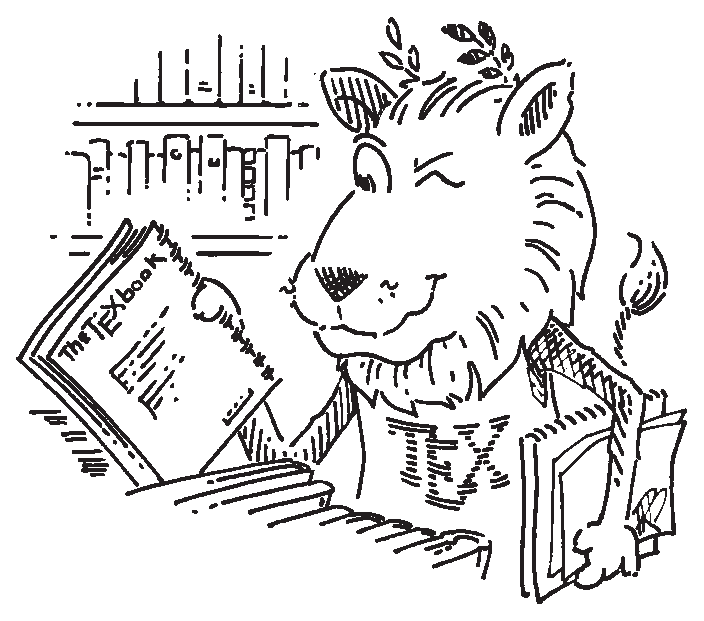
\includegraphics[scale=1.4]{Figure/ctanlion.eps}
        %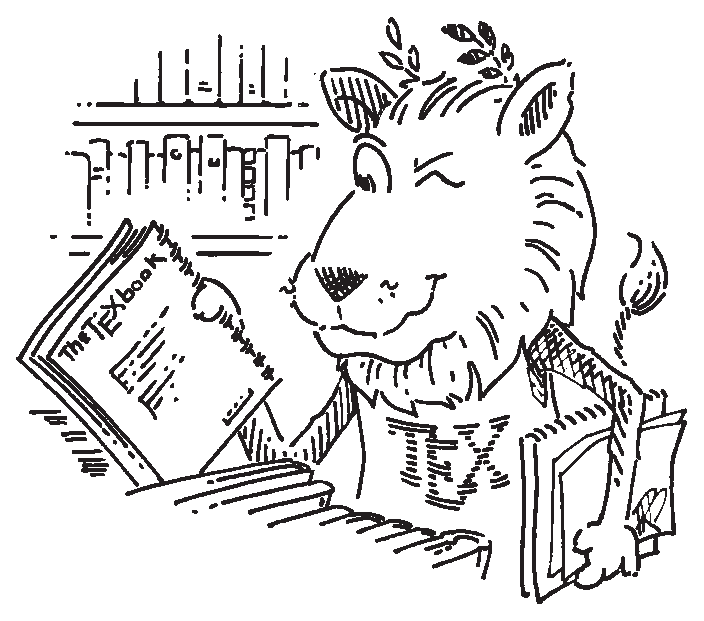
\includegraphics{Figure/ctanlion.eps}
        \begin{center}
            \Huge{\bfseries近世代数引论}\\
            \vspace{15pt}
            \Large\itshape{冯克勤}\\
			\Large\itshape{仅供学习使用,严禁商业使用}
        \end{center}
    \end{titlepage}
    %前言部分
    \frontmatter
    \chapter{修订版前言}\label{prf:1}
这本讲义《近世代数引论》在中国科学技术大学使用了十余年.学生的反映尚好,
主要问题是习题较难.所以我们在书末对于较难的习题增加了提示,同时也补充
了一些新的习题.在内容上去掉“幂零群与可解群”和“$n \geq 5$次一般方程的
根式不可解性”两节,把它们改成两个附录.如果学时不够,正文中某些部分也可
略去不讲或者只做简要介绍.例如伽罗瓦理论可以只介绍基本定理的内容和它的
应用,而不讲证明.对于希洛夫定理、有限生成阿贝耳群的结构、唯一因子分解
整环等内容也可以类似地处理.\par

\chapter{前言}\label{prf:2}
近世代数是讲述群、环、域(以及模)等代数对象基本性质的一门大学课程.它
是今后学习和研究代数学的基础,也是研究其他数学、物理学和计算机科学等不
可缺少的工具.\par
本书是我们于1982年在中国科技大学授课讲义基础上,经过五年教学实践改写而
成.原讲义共五章,为了在一学期(周四学时)内讲完,这次删去了模论和线性
代数两章.\par
近世代数从它产生的年代起就明显有别于古典代数学.它的主要研究对象不是代
数结构中的元素特性,而是各种代数结构本身和不同代数结构之间的相互联系
(同态).掌握近世代数中所体现的丰富的数学思想和方法,比背诵一些代数学
定义和名词字典要重要得多.我们在教学中几乎用半个学期讲述第一章群论,这
是因为在群论中体现了近世代数的基本研究思想和方法,而这些思想和方法在学
生过去学习中是不熟悉的.群论中的定理基本上可分为定量和定性两类:前者的
典型例子是拉格朗日定理,后者的典型例子是同态基本定理.我们着重讲授定性
内容,特别是同态基本定理和群在集合上的作用,这是群论的关键所在.\par
第二章讲述环论和域论初步,正文中的内容是标准的.但是在几个附录中,我们
介绍了在数学发展中有历史意义的几个课题(高斯二平方和问题,代数基本定理
,尺规作图,三等分角等),最后一章向学生展示关于域的有限伽罗瓦扩张的优
美理论.\par
最后,我们向过去几年里对此书的前身提供意见的许多学者、教师和学生表示深
深的谢意,我们也欢迎大家今后对此书给予更多的批评和指正.\par
    %正言部分(分章节)
    \mainmatter
    \tableofcontents
    %第一章
    %Produce by:JJK
%正文部分Chapter1.1
\chapter{群}\label{chap:1}
\section{集合论预备知识}\label{sec:1.1}
群是集合上赋予某种二元运算的一种代数结构.所以在讲述什么是群之前,先要
介绍集合论中我们所需要的一些预备知识.\par
一些特定的对象放在一起就叫做一个\textbf{集合}.例如全体正整数构成一个
集合,表示成~$\mathbb{N}$~.全体整数构成整数集合,表示成~$\mathbb{Z}$~.
类似地有复数集合~$\mathbb{C}$~,实数集合~$\mathbb{R}$~,有理数集合
$\mathbb{Q}$~等等.集合~$A$~中每个对象~$a$~叫做~$A$~中的
\textbf{元素},表示成~$a\in A$~,说成~$a$~属于~$S$~.否则
,如果某个对象~$b$~不属于~$A$~,则表示成~$b\notin A$~.
\par
设~$A$~和~$B$~是两个集合,如果~$A$~中每个元素均是~$B$~中元素,即
\begin{equation*}
    a \in A \Rightarrow a \in B.
\end{equation*}
则~$A$~叫做~$B$~的一个\textbf{子集},表示成~$A\subseteq B$~或者
~$B\supseteq A$~.如果~$A\subseteq B$~并且~$B\subseteq A$~,即
\begin{equation*}
    a \in A \Leftrightarrow a \in B,
\end{equation*}
这也相当于说集合~$A$~与~$B$~包含同样的元素,这时叫做集合~$A$~与
~$B$~相等,表示成~$A=B$~.如果~$A$~是~$B$~的子集并且不等于~$B$~
,则~$A$~叫~$B$~的\textbf{真子集},表示成~$A \subset B$~或者
~$B \supset A$~.不包含任何元素的集合叫做\textbf{空集},表示成
$\varnothing$.空集显然是每个集合的子集.\par
可以有许多方式来表达一个确定的集合.例如若集合~$A$~只有限多(不同)
元素~$a_1,\cdots,a_n(n \in \mathbb{N})$~,则这个集合可表成
\begin{equation*}
    A=\{a_1,\cdots,a_n\}.
\end{equation*}
只有有限多个元素的集合叫\textbf{有限集},否则叫\textbf{无限集}
.具有~$n$~个元素的集合叫~$n$~\textbf{元集},元素个数表示成
~$|A|=n$~.在一般情形下,集合~$\bm{S}$~中具有某种性质~$P$~的
全体元素构成的集合通常表成
\begin{equation*}
    \{x \in \bm{S}~|~x~\mbox{有性质}~P\}.
\end{equation*}
例如:偶数集合~$\{0,\pm2,\pm4,\cdots\}$~可以表成
\begin{equation*}
    \{n \in \bm{Z}~|~n \equiv 0(\mathrm{mod}~2)\}.
\end{equation*}\par
由一些已知集合构作新的集合通常用集合上的运算来实现.下面是集合
的一些最基本运算.设~$A$~和~$B$~是两个集合,它们的公共元素组成
的集合叫做~$A$~和~$B$~的\textbf{交},表示成~$A \cap B$~,即
\begin{equation*}
    A \cap B = \{x~|~ x \in A~\mbox{并且}~x \in B\}.
\end{equation*}
类似地,~$n$~个集合~$A_1,\cdots,A_n$~的交为
\begin{equation*}
    \bigcap_{i=1}^{n}A_i=A_1 \cap A_2 \cap \cdots \cap A_n = 
    \{x~|~x \in A_i,1 \leq i \leq n\}.
\end{equation*}
更一般地,对于任意多个集合形成的集族~$\{A_i~|~i \in I\}$~(其中
$I$~是一个集合,叫该集族的\textbf{下标集合},对于每个~$i \in I$~
,~$A_i$~是该集族中的一个集合),它们的交为
\begin{equation*}
    \bigcap_{i \in I}A_i = \{x~|~x \in A_i,\mbox{对每个}~i \in I\}.
\end{equation*}\par
第二个集合运算是集合的\textbf{并},集合~$A$~与~$B$~的并表示
成~$A \cup B$~,定义为
\begin{equation*}
    A \cup B = \{x~|~x \in A~\mbox{或者}~x \in B\}.
\end{equation*}
类似地:
\begin{equation*}
    \bigcup^n_{i=1}A_i=A_1 \cup A_2 \cup \cdots \cup A_n = \{
x~|~x \in A_i,\mbox{对某个}~i \in I\}.
\end{equation*}
设~$A$~是~$B$~的子集,则~$B-A=\{x~|~x \in B,x \notin A\}$~叫做子
集~$A$~(关于B)的\textbf{补集}.如果在讨论问题中所涉及的集合均是某个
固定集合~$\varOmega$~的子集,则~$\varOmega-A$~也常常简称作~$A$~的
补集,表示成~$\bar{A}$~.\par
设~$A$~和~$B$~是两个集合,我们把集合
\begin{equation*}
    A \times B = \{(a,b)~|~a \in A,b \in B\}
\end{equation*}
叫做~$A$~和~$B$~的直积.在~$A \times B$~中,~$(a,b)=(a',b')$~当且
仅当~$a=a'$~并且~$b=b'$~.类似可定义多个集合的直积
\begin{equation*}
    A_1 \times \cdots \times A_n = \prod^n_{i=1}A_i=\{(a_1,
    \cdots,a_n)~|~a_i \in A_i,1 \leq i \leq n\}.
\end{equation*}
\begin{equation*}
    \prod_{i \in I}A_i = \{(a_i)_{i \in I}~|~a_i \in A_i,
    \mbox{对每个}~i \in I\}
\end{equation*}
为了比较不同的集合,需要将不同集合发生联系,这就是集合之间的映射.
~$f$~叫做从集合~$A$~到集合~$B$~的\textbf{映射},是指对每个
~$a \in A$~均有确定办法给出集合~$B$~中唯一的对应元素,这个对应
元素叫做~$a$~在映射~$f$~之下的象,表示成~$f(a)$~.而“~$f$~把
~$a$~映成~$f(a)$~”这件事表示成~$a \rightarrow f(a)$~.从~$A$~
到~$B$~的映射~$f$~表示成~$f:A \rightarrow B$~或者
~$A \xrightarrow{f} B$~.
设~$f:A \rightarrow B$~和~$g:B \rightarrow C$~都是集合之间的
映射.则可经过连续作用,得到一个从~$A$~到~$C$~的映射
\begin{equation*}
    g \circ f:A \rightarrow C,\quad (g \circ f)(a)=g(f(a)).
\end{equation*}
映射~$g \circ f$~叫做~$f$~与~$g$~的\textbf{合成}映射.\par
设~$f$~和~$g$~均是从集合~$A$~到集合~$B$~的映射,我们称~$f$~
和~$g$~相等(表示成~$f=g$),是指对于每个~$a \in A$~,均有
~$f(a)=g(a)$~.\par
\begin{yinli}\label{yl:1.1.1}
    (合成运算满足结合律)设~$f:A \rightarrow B,~g:B 
    \rightarrow C,~h:C \rightarrow D$~均是集合的映射,则
    \begin{equation*}
h \circ (g \circ f)=(h \circ g) \circ f.
    \end{equation*}
\end{yinli}
\begin{proof}
    对于~$a \in A$~,令~$f(a)=b,g(b)=c,h(c)=d.$~则\par
    \center{$(g \circ f)(a)=c,~(h \circ g)(b)=d.$于是}\par
    \center{($h \circ (g \circ f))(a)=h(c)=d,((h \circ g) 
    \circ f)(a)=(h \circ g)(b)=d.$}
\end{proof}\par
设~$f:A \rightarrow B$~是集合的映射.对于~$A$~的每个子集~$A'$~,令
\begin{equation*}
    f(A')=\{f(x)~|~x \in A'\},
\end{equation*}
这是~$B$~的子集,叫做~$A$~在~$f$~之下的\textbf{象}.另一方面,
对于~$B$~的子集~$B'$~,令~$f^{-1}(B')=\{x \in A~|~f(x) \in B'\}$~
,这是~$A$~的子集,叫做~$B'$~的原象.如果~$f(A)=B$~,即~$B$~中每个元
素均是~$A$~中某个元素(在~$f$~之下)的象,则~$f$~叫做\textbf{满射}.另
一方面,如果~$A$~中不同元素被~$f$~映成~$B$~中不同元素,即:
~$a,~a' \in A,~a \neq a' \Rightarrow f(a) \neq f(a')$~,则~$f$~叫
做单射.最后,若~$f:A \rightarrow B$~同时是单射和满射,则~$f$~叫做
\textbf{一一映射}或\textbf{一一对应}.例如:将集合~$A$~中每个元素均
映成其自身的映射
\begin{equation*}
    1_A:A \rightarrow A,~1_A(a)=a.
\end{equation*}
就是~$A$~到~$A$~的一一对应.映射~$1_A$~叫做集合~$A$~的恒等映射.通常
采用下面引理来判断一个映射是否为一一对应.
\begin{yinli}\label{yl:1.1.2}
    映射~$f:A \rightarrow B$~是一一对应的充分必要条件是存在映射
    ~$g:B \rightarrow A$~,使得~$f \circ g=1_B,g \circ f=1_A$~.
\end{yinli}
\begin{proof}
    如果~$f$~是一一对应,由定义知这意味着对每个~$b \in B$~,均存在唯
    一的~$a \in A$~使得~$f^{-1}(b)=a$~(存在性由于~$f$~是满射,唯一性
    由于~$f$~是单射)于是可定义映射
    \begin{equation*}
        g:B \rightarrow A,~g(b)=f^{-1}(b).
    \end{equation*}
    直接验证~$g \circ f=1_A$~和~$f \circ g=1_B$~;成立.\par
    另一方面,如果~$f$~不是满射,则存在~$b \in B$~,使得
    ~$f^{-1}(b)=\varnothing$~.所以对每个映射~$g:B \rightarrow A$~,
    均有~$(f \circ g)(b)=f(g(b) \neq b$~.于是~$f \circ g \neq 1_B$~.
    如果~$f$~不是单射,则存在~$a,~a' \in A,~a \neq a'$~,使得~$f(a)=
    f(a')=b$~.那么对于每个映射~$g:B \rightarrow A,(g \circ f)(a)=g(b)=(g \circ f)
    (a'),$~于是~$g \circ f \neq 1_A$~.所以若存在~$g:B \rightarrow A$~
    使得~$f \circ g=1_B$~并且~$g \circ f=1_A$~.则必然~$f$~是一一对应.
\end{proof}
当~$f:A \rightarrow B$~是一一对应时,满足~$f \circ g=1_B$~和
~$g \circ f=1_A$~的映射~$g:B \rightarrow A$~是唯一的.这是因为:
若~$g:B \rightarrow A$~也有性质~$f\circ g'=1_B,g'\circ f=1_A,$~
则~$g'=g' \circ 1_B=g'\circ (f\circ g)=(g'\circ f)\circ g=1_A\circ g=g.$~
我们将这个唯一存在的映射~$g$~叫做~$f$~的逆映射,表示成~$f^{-1}$~.\par
设~$A$~是集合,集合~$A \times A$~的每个子集~$R$~叫做集合~$A$~上的一个
\textbf{关系}.如果~$(a,b)\in R$~,便称~$a$~和~$b$~有关系~$R$~,写成~$aRb$~.
例如~$\RR\times \RR$~中子集
\begin{equation*}
    R=\{(a,b)\in \RR\times \RR~|~a~\mbox{比}~b~\mbox{大}\}
\end{equation*}
则实数~$a$~和~$b$~有关系~$R$~即指~$a$~比~$b$~大,这就是“大于”关系.通常将
这个关系记成~$a>b$~.同样还有~$\RR$~上的关系~$\geq$~(大于或
等于),~$<$~(小于),~$\leq$~(小于或等于),~$=$~(等于).集合~$A$~上的关系
$\sim$~叫做\textbf{等价关系},是指它满足如下三个条件:\par
(1)自反性:~$a \sim a$~(对于每个~$a \in A$~)\par
(2)对称性:若~$a \sim b$,则~$b \sim a$.\par
(3)传递性:若~$a \sim b,~b \sim c,$~则~$a \sim c$.\par
设~$\sim$~是集合~$A$~上的等价关系.如果~$a \sim b$~,由对称性知~$b \sim a$
.这时称元素~$a$~和~$b$~等价.对于每个~$a \in A$,以~$[a]$~表示~$A$~中与
$a$~等价的全部元素构成的集合,即
\begin{equation*}
    [a]={\{b \in A~|~b \sim a\}}.
\end{equation*}
由自反性知~$a \in [a]$~,称~$[a]$~为~$a$~所在的等价类,由传递性可知同一等
价类中任意二元素彼此等价(设~$b,c\in [a]$~,则~$b \sim a$,~$a \sim c$~,于是
~$b \sim c$~).不同等价类之间没有公共元素(为什么?)因此集合~$S$~是一些等价类
~$\{[a_i]|i \in I\}$~的并,而这些等价类是两两不相交的.我们从每个等价类~$[a_i]$~
中取出一个元素~$b$~;(即~$b_i \in [a_i]$~),则~$R=\{b_i|i \in I\}$~具有如下
性质:~$A$~中每个元素均等价于某个~$b$~,而不同的~$b$~彼此不等价.我们把具有这
样性质的~$R$~叫做~$S$~对于等价关系~$\sim$~的完全代表系.于是
\begin{equation}
    A=\bigcup_{a \in R}[a](\mbox{两两不相交之并}). \tag{$\ast$}\label{eq:1.1*}
\end{equation}
一般地,若集合~$A$~是它的某些子集~$\{A_i|i \in I\}$~之并,并且~$A$~;两两不相交
,便称~$\{A_i|i \in I\}$~是集合~$S$~的一个\textbf{分拆}.如上所述,~$S$~上的每个等价关系
给出集合~$A$~的一个分拆\eqref{eq:1.1*}.反过来,如果~$\{A_i|i \in I\}$~是集合~$A$~
的一个分拆,可如下定义~$A$~上一个关系:对于~$a,b \in A,$~
\begin{equation*}
    a \sim b \Leftrightarrow a~\mbox{和}~b~\mbox{在同一}~A_i~\mbox{之中},
\end{equation*}
请读者证明这是等价关系.以~$E$~表示~$A$~的全部等价关系,以~$P$~表示~$A$~的全部分拆
,则上面由等价关系到分拆的映射~$f:E \rightarrow P$~和从分拆到等价关系的映射
~$g:P \rightarrow E$~满足~$f \circ g=1_P,~g \circ f=1_E$~,从而~$f$~是一一对应
\thmref{yl:1.1.2}.换句话说,集合A上的等价关系和A的分拆是一一对应的.\par
例如,设~$F$~是由某些集合构成的集族.在~$F$~上定义如下的关系:对于~$A,B \in F$~,
\begin{equation*}
    A \sim B \Leftrightarrow \mbox{存在从~$A$~到~$B$~的一一对应}.
\end{equation*}
这是~$F$~上的等价关系(自反性:~$1_A:A \rightarrow A$~是一一对应,从而~$A \sim A$~.
对称性:若~$f:A \rightarrow B$~是一一对应,则~$f^{-1}:B \rightarrow A$~是一一对应,
从而~$A \sim B \Rightarrow B \sim A$~.传递性基于习题\ref{xiti:1.1.3}.)对于这
种等价关系,彼此等价的集合叫做是\textbf{等势}的.比如说,两个有限集合等势(即存在一一
对应)的充要条件是它们有同样多元素,即~$|A|=|B|$.与正整数集合~$N$~等势的集合叫做
\textbf{可数无限集合},其他无限集合叫做\textbf{不可数集合}.熟知实数集合~$R$~是不可
数集合.而正偶整数的全体~$E$~是可数(无穷)集合,因为存在着一一对应
~$\NN\rightarrow E,~n \rightarrow 2n$.这个例子也表明,无限集合~$A$~
的一个真子集可以与~$A$~等势!\par
设~$A$~是集合.从~$A \times A$~到~$A$~的映射
\begin{equation*}
    f:A \times A \rightarrow A
\end{equation*}
叫做集合A上的一个(二元)运算.例如:通常复数加法就是运算
\begin{equation*}
    f:\CC \times \CC \rightarrow \CC,~f(\alpha,\beta)=\alpha+\beta.
\end{equation*}
我们经常把集合~$A$~上的运算表示成~$\cdot$,即对于~$a,b \in A,~f(a,b)$~
写成~$a \cdot b(\in A)$~或者更简单写成~$ab$.\par
运算~$\cdot$~叫做满足结合律,是指
\begin{equation*}
    a \cdot (b \cdot c)=(a \cdot b) \cdot c(\mbox{对任意~$a,b,c \in A$}).
\end{equation*}
运算~$\cdot$~叫做满足交换律,是指
\begin{equation*}
    a \cdot b=b \cdot a(\mbox{对任意~$a,b \in A$}).
\end{equation*}
一个集合赋予满足某些特定性质的(一个或多个)二元运算,便得到各种代数结构.
本书讲述群、环和域三种代数结构.

%习题1.1\label{xiti:1.1}
\xiti
\begin{enumerate}
    \item 设~$B,A_i(i \in )$~试证:\label{xiti:1.1.1}
    \begin{enumerate}
        \item B $\cap\left(\bigcup_{i \in I}A_i\right)=\bigcup_{i \in I}(B\cap A_i),$
        \item B $\cup\left(\bigcap_{i \in I}A_i\right)=\bigcap_{i \in I}(B\cup A_i),$
        \item $\overline{\bigcup_{i \in I}A_i}=\bigcap_{i \in I}\overline{A_i},~
        \overline{\bigcap_{i \in I}A_i}=\bigcup_{i \in I}\overline{A_i}.$
    \end{enumerate}
    \item 设~$f:A \rightarrow B$~是集合的映射,~$A$~是非空集合.试证:\label{xiti:1.1.2}
    \begin{enumerate}
        \item ~$f$~为单射~$\Leftrightarrow$~存在~$g:B \rightarrow A$,使得~$g \circ f=1_A$~.
        \item ~$f$~为满射~$\Leftrightarrow$~存在~$h:B \rightarrow A$.使得~~$f \circ h=1_B$~.
    \end{enumerate}
    \item 如果~$f:A \rightarrow B,~g:B \rightarrow C$~均是一一对应,则~$g \circ f:A \rightarrow C$~也是一一对应,且~$(g \circ f)^{-1}=f^{-1} \circ g^{-1}$.\label{xiti:1.1.3}
    \item 设~$A$~是有限集,~$P(A)$~是~$A$~的全部子集(包括空集)所构成的集族,试证~$|P(A)|=2^{|A|}$.换句话说,~$n$~元集合共有~$2^n$~个不同的子集.\label{xiti:1.1.4}
    \item 设~$f:A \rightarrow B$~是集合的映射.在集合~$A$~上如下定义一个关系:对任意~$a,a' \in A,~a \sim a'$~当且仅当~$f(a)=f(a')$.试证,这样定义的关系是一个等价关系.\label{xiti:1.1.5}
    \item 证明等价关系的三个条件是互相独立的,也就是说,已知任意两个条件不能推出第三个条件.\label{xiti:1.1.6}
    \item 设~$A,B$~是两个有限集合.\label{xiti:1.1.7}
    \begin{enumerate}
        \item $A$~到~$B$~的不同映射共有多少个?
        \item $A$~上不同的二元运算共有多少个?
    \end{enumerate}
\end{enumerate}
    \section{什么是群}\label{sec:1.2}
让我们先从半群讲起.
\begin{Definition}
    集合~$S$~和~$S$~上满足结合律的二元运算~$\cdot$~所形成的代数结构叫做\textbf{半群}.
    这个半群记成~$(S,\cdot)$~或者简记成~$S$,运算~$x \cdot y$~也常常简写成~$xy$~.
\end{Definition}\par
如果运算又满足交换律,则~$(S,\cdot)$~叫做\textbf{交换半群}.象通常那样令
~$x^2=x \cdot x,~x^{n+1}=x^n \cdot x(=x \cdot x^n~,~n \geq 1)$
\begin{Definition}
    设~$S$~是半群,元素~$e \in S$~叫做半群~$S$~的幺元素,是指对每个~$x \in S,~xe=ex=x.$~
\end{Definition}
如果半群~$S$~有幺元素~$e$~,则它是唯一的,因若~$e'$~也是幺元素,则~$e'=e'e=e$~.我们将半群~$S$~中这个
唯一的幺元素(如果存在的话)通常记作~$1_S$~或者~$1$~具有幺元素的半群叫\textbf{含幺半群}.
\begin{Definition}
    设~$S$~是含幺半群.元素~$y \in S$~叫做元素~$x \in S$~的逆元素,是指~$xy=yx=1$.
\end{Definition}
如果~$x$~有逆元素,则它一定唯一.因为若~$y'$~也是~$x$~的逆元素,则~$xy'=y'x=1$.于是
\begin{equation*}
    y=y \cdot 1=y(xy')=(yx)y'=1 \cdot y'=y'.
\end{equation*}
所以若~$x$~具有逆元素,我们把这个唯一的逆元素记作~$x^{-1}$~,则~$xx^{-1}=x^{-1}x=1$~.
\begin{Definition}
    定义半群~$G$~如果有幺元素,并且每个元素均可逆,则~$G$~叫做群.此外,若运算又满足交换律,则~$G$~叫
    做\textbf{交换群}或叫\textbf{阿贝耳(Abel)群}.
\end{Definition}
下面给出半群和群的一些例子.
\begin{example}
    设~$M$~为非负整数全体,~$(M,+)$~是含幺交换半群,幺元素是数~$0$~,但它不是群,因为只有~$0$~对于
    加法在~$M$~中才可逆.
\end{example}\par
$\ZZ,\QQ,\RR,\CC$~对于加法均是阿贝耳群,叫做整数加法群,有理数加法群等等.\par
$(\NN,~\cdot~)$~是含幺交换(乘法)半群,幺元素为~$1$~.它不是群.令~$\QQ\ast$~为非零有理数全体,
则~$(\QQ\ast,~\cdot~)$~是交换群,幺元素为~$1$~,非零有理数~$a$~的乘法逆为~$a^{-1}$~.这叫非零
有理数乘法群,同样有~$(\RR\ast,~\cdot~)$~和~$(\CC\ast,~\cdot~)$~,这些都是阿贝耳群.
\begin{example}
    以~$M_{m,n}(\CC)$~表示全体~$m$~行~$n$~列复矩阵组成的集合,它对矩阵加法形成阿贝耳群.幺元素是全零矩阵,
    而矩阵~$A=(a_{ij})$~的加法逆是~$-A=(-a_{ij})$~.以~$M_n(\CC)$~表示~$n$~阶复方阵全体,它对乘法形成含
    幺半群,幺元素是单位方阵~$I_n$.由线性代数可知,~$n$~阶复方阵~$A$~有乘法逆的充要条件是~$\det A \neq 0$
    .从而~$M_n(\CC)$~不是群,并且当~$n \geq 2$~时,易知半群~$M_n(\CC)$~不是交换的.类似有加法交换群
    ~$M_{m,n}(\RR)$~,含幺半群~$M_{n}(\QQ)$~等等.
\end{example}
\begin{example}
    设~$A$~是非空集合,以~$\sum(A)$~表示从~$A$~到~$A$~全体映射组成的集合.则~$\sum(A)$~对于映射合成运算
    形成含么半群.幺元素为~$A$~上恒等映射~$1_A$~.由1.1的\thmref{yl:1.1.2}可知,~$\sum(A)$~中映射~$f$~
    可逆的充要条件是~$f$~为一一对应.所以当~$|A|>1$~时,~$\sum(A)$~不是群,并且半群~$\sum(A)$~不是交换的.
\end{example}
\begin{example}
    欧氏平面~$\RR^2$~中保持欧氏距离不变的运动叫做\textbf{欧氏运动}.由于欧氏运动必为~$\RR^2$~到自身之上
    的一一对应,并且它的逆仍是欧氏运动,而两个欧氏运动的合成仍是欧氏运动,从而全体欧氏运动形成群,叫做平面
    上的\textbf{欧氏运动群},这也是非阿贝耳群.
\end{example}
\begin{example}
    设~$n$~为正整数,我们在~$\ZZ$~上定义如下关系:对于整数~$a$~和~$b$~,
    \begin{equation*}
        a \sim b \Leftrightarrow n~|~a-b(\mbox{即}~a \equiv b(\mathrm{mod}~n)) 
    \end{equation*}
    易知这是等价关系,于是整数集合~$\ZZ$~分拆成~$n$~个等价类:~$\bar{0},\bar{1},\cdots,\overline{n-1}$~,
    其中~$\bar{i}$~表示~$i$~所在的等价类,即~$\bar{i}=\{m \in \ZZ~|~m \equiv i(\mathrm{mod}~n)\}$~.而
    ~$\{0,1,2,\cdots,n-1\}$~是~$Z$~对于上述模~$m$~同余关系的一个完全代表系.\par
    以~$Z_n$~表示上述~$n$~个等价类组成的集合.在~$Z_n$~上定义加法:
    \begin{equation*}
        \bar{a}+\bar{b}=\overline{a+b}
    \end{equation*}
    由同余式基本性质可知这个加法运算是可以定义的,即与等价类(或叫\textbf{模~$n$~同余类})中代表元的取法无关
    ,并且~$Z_n$~对于这个运算形成交换群,幺元素是~$\bar{0}$,这叫\textbf{整数模~$n$~加法群}.\par
    如果~$Z_n$~中定义乘法
    \begin{equation*}
        \overline{a}\overline{b}=\overline{ab}
    \end{equation*}
    则~$Z_n$~对此乘法是含么交换半群,幺元素为~$\bar{1}$~.由于等式~$\bar{a}\bar{b}=\bar{1}$~相当于同余式
    ~$ab \equiv 1(\mathrm{mod}~n)$~.从初等数论知道,对于给定的~$a$~,存在~$b$~满足
    ~$ab \equiv 1(\mathrm{mod}~n)$~的充要条件是~$(a,n)=1$.从而~$a$~对于上述乘法可逆的充要条件是
    ~$(a,n)=1$.
\end{example}
设~$(M,~\cdot~)$~是含幺半群,我们以~$U(M)$~或者~$M*$~表示半群~$M$~中可逆元素全体.
\begin{Definition}
    若~$(M,~\cdot~)$~是含幺半群,则~$(U(M),~\cdot~)$~是群.
\end{Definition}
\begin{proof}
    由~$1_M^{-1}=1_{M}$~可知~$1=1_M \in U(M)$~.若~$a,b \in U(M)$~,则~$a,b$~均可逆,易知~$b^{-1}a^{-1}$~
    是~$ab$~的逆元素,从而~$ab \in U(M)$~.因此~$\cdot$~是~$U(M)$~上的二元运算.这运算在~$U(M)$~中当然
    也满足结合律,于是~$(U(M),~\cdot~)$~是含幺半群.由于~$U(M)$~中每个元素~$a$~均可逆,从而~$a^{-1} \in M$~
    也可逆(因为~$a$~是~$a^{-1}$~的逆),因此~$a^{-1} \in U(M)$~.从而~$U(M)$~中每个元素在~$U(M)$~中均
    可逆.根据定义,~$U(M)$~为群.
\end{proof}
于是由前面的例子便知:\par
\begin{enumerate}
    \item 全体~$n$~阶可逆复方阵形成乘法群,叫做复数上的~$n$~次\textbf{一般线性群},表示成~$GL(n,\CC)$~.同样有群~$GL(n,\RR)$,\par
    $GL(n,\QQ)$~等.
    \item 设~$A$~为非空集合,~$A$~到自身之上的所有一一对应对于合成运算形成群,叫做集合~$A$~上的\textbf{对称群}或\textbf{全置换群},表示成~$S(A)$~,其中元素(即~$A$~到~$A$~的一一对应)叫做集合~$A$~上的\textbf{置换}.
    \item 设~$n$~为正整数,~$\bar{a}$~为整数~$a$~的模~$n$~同余类.则集合则集合
    \begin{equation*}
        Z^*_n = \{\bar{a}~|~(a,n)=1\}
    \end{equation*}
\end{enumerate}
对于乘法形成阿贝耳群.这个群有~$\varphi(n)$~个元素,其中~$\varphi(n)$~是~$1$~到~$n$~中与~$n$~互素的整数个数($\varphi(n)$~叫\textbf{欧拉函数}).\par
设~$G$~是群.若集合~$G$~有限,称~$G$~为有限群,否则叫无限群.若有限群~$G$~共有~$n$~个元素,则~$G$~叫~$n$~\textbf{阶群}或叫~$n$~\textbf{元群},~$n=|G|$~叫有限群~$G$~的\textbf{阶}.\par
为了考查各种群之间的联系,我们要研究群之间的映射.但是群不仅是集合还有运算,所以我们需要映射与群运算保持协调.确切地说:
\begin{Definition}
    设~$(G,\cdot)$~和~$(G',\circ)$~是两个群.映射~$f:G \to G'$~叫做群~$G$~到群~$G'$~的同态,是指对~$a,b\in G$~
\end{Definition}
$f(a \cdot b) = f(a) \circ f(b)$(简记为~$f(ab)=f(a)f(b)$).
此外,若~$f$~又为单射或满射,则~$f$~分别叫\textbf{单同态}或\textbf{满同态}.如果同态~$f$~是一一对应,则称~$f$~是群~$G$~到群~$G'$~的同构.这时,称群~$G$~和~$G'$~是同构的,表示成~$G=G'$~或者~$f:G\underrightarrow{\sim}G'$~.

\newpage
\begin{figure}[htbp]
    \centering
    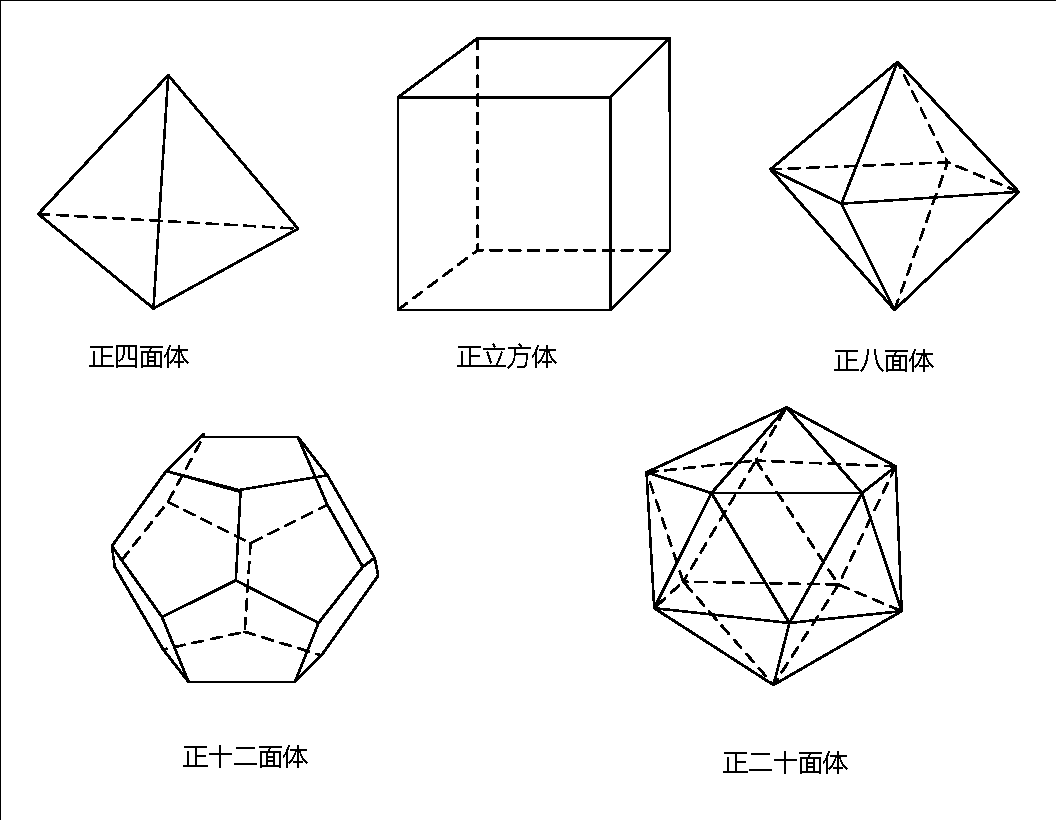
\includegraphics[scale=0.6]{Figure/old/2.pdf}
    \caption{}\label{fig:2}
\end{figure}

\begin{figure}[htb]
    \centering
    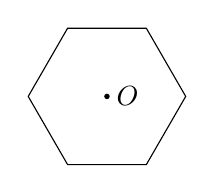
\begin{tikzpicture}
        \draw (0,0) -- (0.5,0.866) -- (1.5,0.866) -- (2,0)
         -- (1.5,-0.866) -- (0.5,-0.866) -- cycle;
        \fill (1,0) circle[radius=1pt] node[right] {$O$};
    \end{tikzpicture}
    \caption{正六边形}
\end{figure}

    %第二章
    %第三章
\end{document}
